\documentclass[12pt, twoside]{article}
\usepackage[letterpaper, margin=1in, headsep=0.5in]{geometry}
\usepackage[english]{babel}
\usepackage[utf8]{inputenc}
\usepackage{amsmath}
\usepackage{amsfonts}
\usepackage{amssymb}
\usepackage{tikz}
\usetikzlibrary{quotes, angles}
\usepackage{graphicx}
\usepackage{enumitem}
\usepackage{multicol}
\usepackage{hyperref}

\newif\ifmeta
\metatrue %print standards and topics tags

\title{IB Mathematics}
\author{Chris Huson}
\date{March 2022}

\usepackage{fancyhdr}
\pagestyle{fancy}
\fancyhf{}
\renewcommand{\headrulewidth}{0pt} % disable the underline of the header
\raggedbottom

\fancyhead[LE]{\thepage}
\fancyhead[RO]{\thepage \\ Name: \hspace{4cm} \,\\}
\fancyhead[LO]{BECA / IB Math 6 Geometry \\* 17 March 2022}

\begin{document}
\subsubsection*{6.3 The Law of Sines}
\begin{enumerate}
\item The following diagram shows triangle $ABC$, with $A\hat{B}C=60^\circ$, $A\hat{C}B=25^\circ$, and $BC=8$ cm. \\[0.25cm]
Find $AB$. \hfill \emph{diagram not to scale}
  \begin{flushright}
    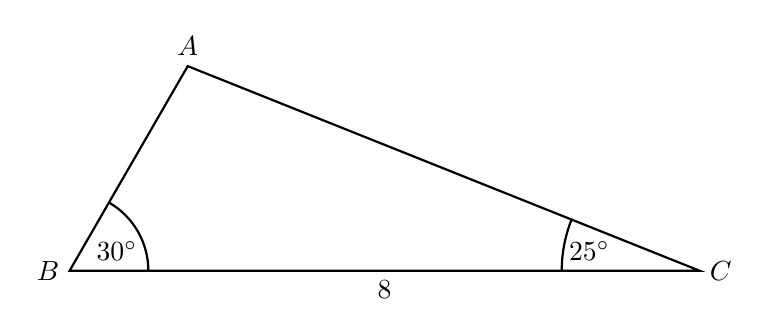
\begin{tikzpicture}[scale=1]
      \draw [thick](60:3)node[above]{$A$}--
      (0,0)node[left]{$B$}--
      (0:8)node[right]{$C$}--cycle;
      \node at (0:4)[below]{$8$};
      \draw [thick, -] (0:1) arc [start angle=0, end angle=60, radius=1];
      \node at (0:0.6)[above]{$30^\circ$};
      \draw [thick, -] (0:6.25) arc [start angle=180, end angle=158, radius=1.75];
      \node at (0:6.6)[above]{$25^\circ$};
    \end{tikzpicture}
  \end{flushright}\vspace{2cm}

\item The following diagram shows triangle $PQR$. \\[0.25cm]
$Q\hat{R}P=45^\circ$, $P\hat{Q}R=30^\circ$, and $PQ=13$ cm. \\[0.25cm]
Find $PR$.
  \begin{flushright}
    \begin{tikzpicture}[scale=1]
      \draw [thick](60:6.5)node[above]{$Q$}--
      (0,0)node[left]{$P$}--
      (-45:4.6)node[below]{$R$}--cycle;
      \node at (70:3)[below]{$13$};
      \draw [thick, -] (60:5) arc [start angle=-120, end angle=-90, radius=1.5];
      \node at (55:5.1)[above]{$30^\circ$};
      \draw [thick, -] (-45:3.1) arc [start angle=135, end angle=90, radius=1.5];
      \node at (-41:3.8)[above]{$45^\circ$};
      \node at (60:8)[above]{\emph{diagram not to scale}};
    \end{tikzpicture}
  \end{flushright}

\newpage
\item Consider a circle with centre $O$ and radius 7 cm. Triangle $ABC$ is drawn such that its vertices are on the circumference of the circle. \\[0.25cm]
$AB=12.2$ cm, $BC=10.4$ cm, and $A\hat{C}B=61^\circ$. \\[0.25cm]
Find $B\hat{A}C$.
  \begin{flushright}
    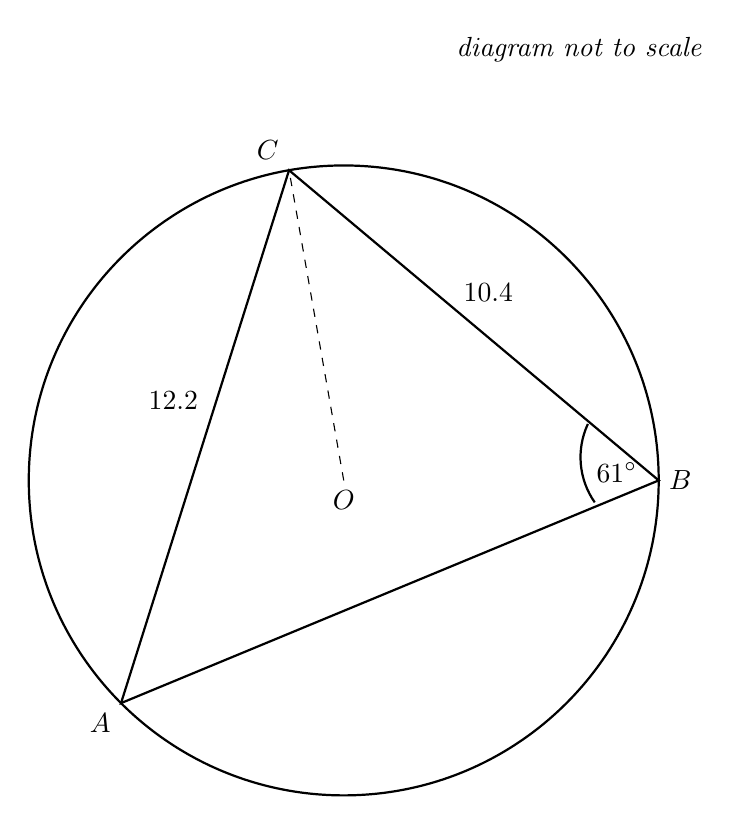
\begin{tikzpicture}[scale=1]
      \draw [thick] (0,0) circle [radius=4];
      \draw [dashed] (0,0)node[below]{$O$}--(100:4);
      \draw [thick](0:4)node[right]{$B$}--
      (100:4)node[above left]{$C$}--
      (-135:4)node[below left]{$A$}--cycle;
      \node at (55:3.2)[below]{$10.4$};
      \node at (150:2.5)[below]{$12.2$};
      \draw [thick, -] (-5:3.2) arc [start angle=215, end angle=155, radius=1];
      \node at (1.5:3.85)[left]{$61^\circ$};
      \node at (60:6)[above]{\emph{diagram not to scale}};
    \end{tikzpicture}
  \end{flushright}

\newpage
\item Triangle $ABC$ has $\hat{A}=40^\circ$, $AB=7 \text{ cm}$, $BC=6 \text{ cm}$. Find the measure of $\hat{C}$:
  \begin{enumerate}
    \item Write down the law of sines, substituting appropriate values.
    \item Solve for the measure of angle $C$
  \end{enumerate}
  \begin{center}
  \begin{tikzpicture}[scale=0.6]
  \draw (0,0) node[anchor=north]{$A$}
    -- (12,0) node[anchor=north]{$C$}
    -- (6.75,6) node[anchor=south]{$B$}
    -- cycle;
    %(0,3) node[anchor=south]{$40^\circ$};
    %\draw [dashed] (1.5,0) -- (1.5,4.2);
  \end{tikzpicture}
  \end{center}

\item Given a circle with radius of one, centered on the origin. An angle with measure $30^\circ$ is placed in standard position. Mark the point $A$, the intersection of the circle and angle ray, as an ordered pair.
    \begin{center}
    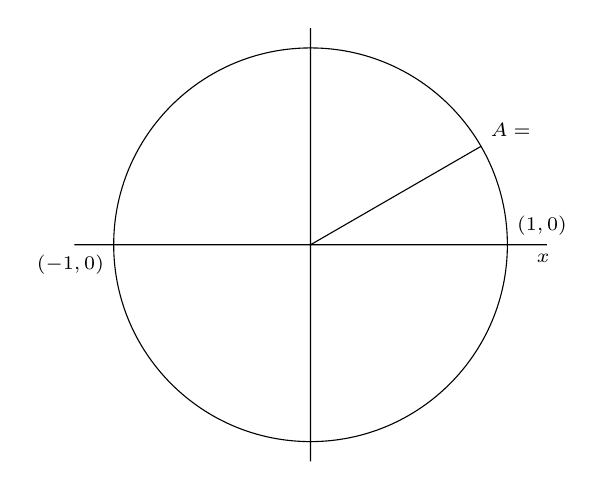
\begin{tikzpicture}[scale=2.5]
      \draw[font=\scriptsize]
        (-1.2, 0) -- (1.2, 0)
        (0, -1.1) -- (0, 1.1)
        (0, 0) -- (0.866, .5) node[above right] {$A=$}
        (0, 0) circle[radius=1]
        (-1, 0) node[below left] {$(-1,0)$}
        (1, 0) node[above right] {$(1,0)$}
        (1.1, 0) node[below right] {$x$}
        ;
    \end{tikzpicture}
    \end{center}
    \begin{enumerate}
          \item Write down the value of $\sin{30^\circ}$\\[0.25in]
          \item  Write down the value of $\cos{30^\circ}$\\[0.25in]
    \end{enumerate}
    
    
    

\end{enumerate}
\end{document}
